%% Copyright 2006-2015 Xavier Danaux (xdanaux@gmail.com).
%
% This work may be distributed and/or modified under the
% conditions of the LaTeX Project Public License version 1.3c,
% available at http://www.latex-project.org/lppl/.


\documentclass[11pt,letterpaper,sans,dvipsnames]{moderncv}        % possible options include font size ('10pt', '11pt' and '12pt'), paper size ('a4paper', 'letterpaper', 'a5paper', 'legalpaper', 'executivepaper' and 'landscape') and font family ('sans' and 'roman')

\usepackage{fancyhdr}
\usepackage{xcolor}
\chead{\color{RoyalBlue}G. S. Antell, PhD}
% \cfoot{Page \thepage\ of \pageref{LastPage}}

% moderncv themes
\moderncvstyle{fancy}                             % style options are 'casual' (default), 'classic', 'banking', 'oldstyle' and 'fancy'
\moderncvcolor{blue}                               % color options 'black', 'blue' (default), 'burgundy', 'green', 'grey', 'orange', 'purple' and 'red'
%\renewcommand{\familydefault}{\sfdefault}         % to set the default font; use '\sfdefault' for the default sans serif font, '\rmdefault' for the default roman one, or any tex font name

% \nopagenumbers{}                                  % uncomment to suppress automatic page numbering for CVs longer than one page

% character encoding
\usepackage[utf8]{inputenc}                       % if you are not using xelatex ou lualatex, replace by the encoding you are using

% adjust the page margins
\usepackage[scale=0.78,top=1in,bottom=1in]{geometry}
%\setlength{\hintscolumnwidth}{3cm}                % if you want to change the width of the column with the dates
%\setlength{\makecvtitlenamewidth}{10cm}           % for the 'classic' style, if you want to force the width allocated to your name and avoid line breaks. be careful though, the length is normally calculated to avoid any overlap with your personal info; use this at your own typographical risks...

\hyphenpenalty=10000

% personal data
\name{Gwen S.}{Antell, PhD}
% \title{Resumé title}             
%\address{Geology 1242 \\ 900 University Ave.}{Riverside, CA 92521}{}% "postcode city" and "country" arguments can be omitted or provided empty
\email{gwen.antell\\@ucr.edu}                           
% \phone[mobile]{}      % the optional "type" of the phone can be "mobile" (default), "fixed" or "fax"
\homepage{gwenantell.com}                    
%\social[linkedin]{john.doe}                 
% \social[twitter]{GwenAntell}        
%\social[github]{GwenAntell}        
% \extrainfo{additional information}    
% \photo[64pt][0.4pt]{Antell_profile_small}              % '64pt' is the height the picture must be resized to, 0.4pt is the thickness of the frame around it (put it to 0pt for no frame) and 'picture' is the name of the picture file
% \quote{Some quote}     

\usepackage[backend=biber, isbn=false, bibstyle=numeric, sorting=none, defernumbers=true, maxbibnames=50]{biblatex} 
\bibliography{presentations_publications.bib}

  
% bibliography with mutiple entries
%\usepackage{multibib}
%\newcites{book,misc}{{Books},{Others}}

%----------------------------------------------------------------------------------
%            content
%----------------------------------------------------------------------------------
\begin{document}

\thispagestyle{empty}

\makecvtitle

\section{Education}
\cventry{2017--2021}{DPhil}{University of Oxford}{UK}{}{Departments of Earth Sciences and Zoology. Defended Jan 2022 with no corrections.}  % arguments 3 to 6 can be left empty
\cventry{2012--2016}{B.S.}{Yale University}{USA}{\textit{magna cum laude}}{Ecology \& Evolutionary Biology (with distinction) and Geology \& Geophysics}

\section{PhD thesis}
\cvitem{Title}{\emph{Macroecological consequences of biotic and abiotic factors in marine communities through time}}
\cvitem{Supervisors}{Erin Saupe (Earth Sciences) \& Tim Coulson (Zoology)}
\cvitem{Research interests}{ % 
\begin{itemize}
\item Biodiversity across spatial, temporal, and taxonomic scales
\item Macroecology, marine biology, and invertebrate paleontology
\item Inferential statistics on time series and spatial data
\end{itemize}
}

\section{Employment}
\cventry{2022--Present}{UC President's Postdoctoral Fellowship Program (PPFP)}{Earth \& Planetary Sciences}{University of California, Riverside}{}{Independent research fellowship; mentorship as part of the diversifying faculty initiative.}

\cventry{2022}{Postdoctoral Research Assistant}{Earth Sciences}{Oxford}{}{Grant-funded by UK Natural Environment Research Council to develop analysis software.}

\cventry{2017--2021}{Graduate teaching assistant}{Earth Sciences}{Oxford}{}{
Labs, discussion sections, and field courses on evolution and past environments}

\cventry{2016--2017}{Geoscientists-in-the-Parks Intern}{US National Park Service, Geologic Resources Division}{Florissant National Monument}{CO}{Published independent research, assisted exhibit design, and surveyed geoheritage resources.}

\cventry{2013--2016}{Collections Assistant}{Yale Peabody Museum of Natural History, Invertebrate Paleontology Division}{New Haven}{CT}{Described new fossil species, cataloged specimens, and hosted public tours.}

% \cventry{2015--2016}{Freshmen Counselor}{Yale College}{New Haven, CT}{}{Academic and personal % advising to freshmen; welfare role under the Dean's office.}
% {Description line 1\newline{}Description line 2}

\section{Leadership}
\cvitem{Divisional Equality, Diversity, \& Inclusion Fellow}{serving the STEM division EDI Steering Group and contributing to Oxford's 3-year strategic plan, 2020--2021.}
\cvitem{Co-chair}{Working group on racial diversity and inclusion in Earth Sciences Dept., Oxford, 2019--2020. Co-authored report of 42 action item recommendations.}
\cvitem{Representative for graduate students}{Equality Committee, Earth Sciences Dept., Oxford, 2017--Present. Changed policies and liaised with students.}
\cvitem{Representative for Earth Sciences}{Divisional Joint Consultative Committee, representing graduate student interests, 2018--2020.}
\cvitem{President}{St John's College, Middle Common Room Committee (graduate student body), 2018--2019; \textbf{Disabled students' officer} 2017--2018.}
\cvitem{Women's Leadership Forum facilitator}{St John's College grad.\ students, 2018.}
%\cvitem{President}{Yale Ecology and Evo.\ Bio.\ Group, 2015--2016; member 2013--2016.}
%\cvitem{Secretary}{Connecticut Entomological Society, 2015--2016; member 2013--2016}

\pagebreak

% bibliography
\nocite{*}
\printbibliography[type=article, title={Publications}] % , resetnumbers=true

\section{Other writing}
% \printbibliography[type=misc, title={Other writing}, resetnumbers=true]
\cvitem{}{(Not peer-reviewed.)}
\cvitem{}{S Greene, \textbf{G Antell}, \textit{et al.} ``Safety and belonging in the field: a checklist for educators.'' \textit{EarthArXiv (2021).} \href{https://doi.org/10.31223/X53P6H}{DOI: 10.31223/X53P6H}.}
\cvitem{}{\textbf{G Antell}. ``All colours of pride.'' Rainbow Research blog series, journal of \textit{Methods in Ecology \& Evolution} (2021). \href{https://methodsblog.com/2021/06/28/rainbow-research-all-colours-of-pride/}{URL: https://methodsblog.com/2021/06/28}.}
\cvitem{}{B Fernando and \textbf{G Antell}. ``Recommendations for improving racial equality, diversity, and inclusion in the Department of Earth Sciences, University of Oxford.'' Public report (2021). Available at: \href{https://www.earth.ox.ac.uk/2020/06/department-of-earth-sciences-releases-report-of-ad-hoc-working-group-on-bame-issues/}{\textit{https://www.earth.ox.ac.uk/2020/06}}.}

\section{Software}
\cvitem{divvy}{Developed and actively maintaining an R package for spatial subsampling of biodiversity data, to facilitate fair comparisons of ecological metrics through time, between clades, or across environments (Antell \textit{et al.} 2020).}
\cvitem{kerneval}{Developed an R package for kernel density estimation that corrects density curves for biased observation/sampling (Antell \textit{et al.} 2021).}
\cvitem{Install at}{\href{https://github.com/GwenAntell/divvy}{github.com/GwenAntell/divvy}; \href{https://github.com/GwenAntell/kerneval}{github.com/GwenAntell/kerneval}}
\hfill 
{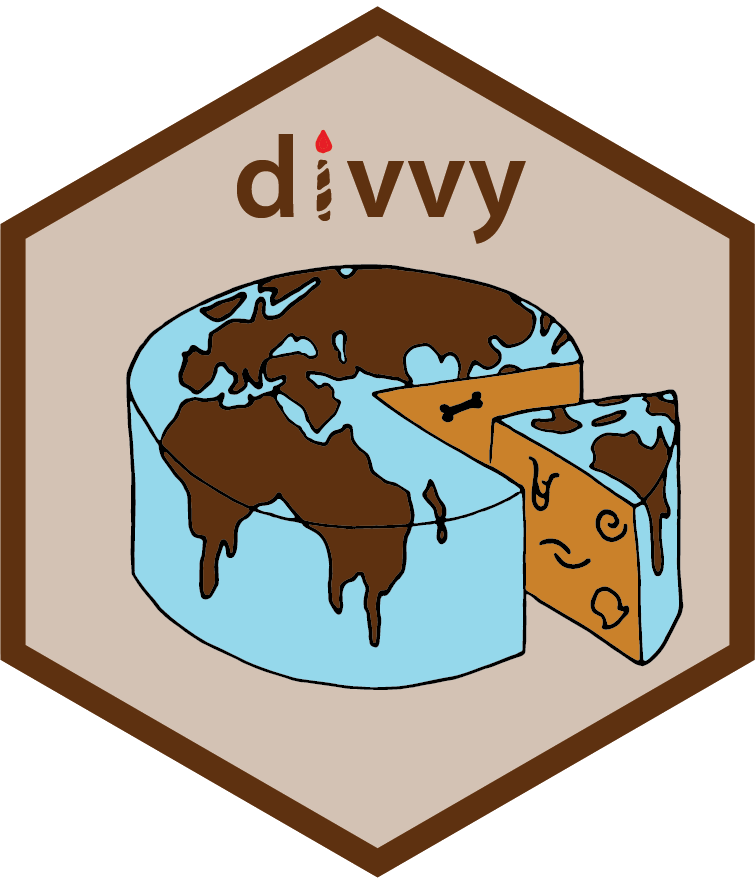
\includegraphics[width=2.3cm]{divvy_logo}}
{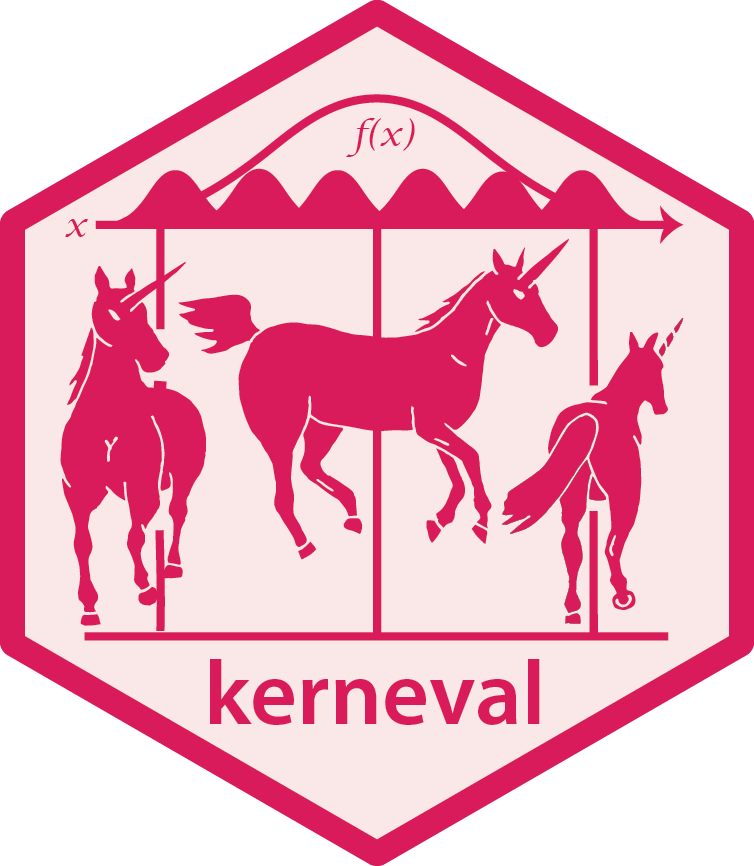
\includegraphics[width=2.3cm]{kerneval_logo}}

\pagebreak

\section{Awards}
\subsection{Scholarships}
\cvitemwithcomment{}{President's Postdoctoral Fellowship, U.\ of California}{2022--}
\cvitemwithcomment{}{Clarendon Fund Scholarship}{2017--2021}
\cvitemwithcomment{}{St John's College Alumni Scholarship}{2017--2021}
\cvitemwithcomment{}{NSF Graduate Research Fellowship Program (declined)}{2017}
\cvitemwithcomment{}{Jerry (1953) and Jackie Inskeep Scholarship Fund}{2013--2016}
\cvitemwithcomment{}{Summer Environmental Fellowship, Yale}{2014}
\cvitemwithcomment{}{US National Merit Scholarship}{2012}
\subsection{Grants}
\cvitemwithcomment{}{Burdett-Coutts Grant, Earth Sciences, of Oxford (\pounds 1,650)}{2019}
\cvitemwithcomment{}{Postgraduate Special Grant, St John's College (\pounds 1,250)}{2018}
\cvitemwithcomment{}{Travel Grant, Palaeontological Association (\pounds 300)}{2018}
\cvitem{}{Ernst Mayr travel grant for animal systematics, Museum of Comparative Zoology, Harvard University (\$1,100) \hspace{18 pc} {\small \textit{2016}}}
% \cvitemwithcomment{}{Pierson College Richter Fellowship (\$500)}{2015}
\cvitemwithcomment{}{Yale Science Center Int'l Fellowship (\$3,870; \$4,300)}{2014, 2015}
\cvitemwithcomment{}{Yale Freshmen Summer STEM Research Fellowship (\$4,300)}{2013}
\subsection{Awards}
\cvitem{}{Winifred Goldring Award for outstanding paleontology PhD student; conferred by Association for Women Geoscientists and Paleontological Society \hspace{4 pc} {\small \textit{2021}}}
\cvitemwithcomment{}{1st-place student talk in Geobiology \& Geomicrobiology, GSA meeting}{2020}
\cvitemwithcomment{}{Oxford Earth Sciences award for equality, diversity, \& inclusion}{2020}
\cvitemwithcomment{}{1st-place student talk, North American Paleontological Convention}{2019}
\cvitem{}{D.\ E.\ Chantler Award for ``the Yale Senior who has best exemplified qualities of courage, strength of character, and high moral purpose'' \hspace{7 pc} {\small \textit{2016}}} % Yale 
\cvitemwithcomment{}{W. R. Belknap Prize for excellence in a biology thesis, Yale}{2016}
\cvitemwithcomment{}{1st-place student speed talk, Connecticut Entomological Society}{2015}
% commended talk, CPEG

\section{Invited talks}
\cvitemwithcomment{Stanford}{Dept.\ of Geological Sciences}{Apr 2023}
\cvitemwithcomment{UC Riverside}{Environmental Dynamics and GeoEcology Institute}{Mar 2023}
\cvitemwithcomment{U.\ of Southern California}{Paleo/Environmental seminar series}{Jan 2023}
\cvitemwithcomment{UC Riverside}{Dept.\ of Earth \& Planetary Sciences}{Jan 2023}
\cvitemwithcomment{UC Los Angeles}{Dept.\ of Earth, Planetary \& Space Science}{Sep 2022}
\cvitemwithcomment{Sheffield University}{Ecology \& Conservation series}{Oct 2021}
\cvitemwithcomment{Yale}{Earth and Planetary Sciences}{May 2021}
\cvitemwithcomment{Harvard}{MCZ and Dept.\ Organismic \& Evo.\ Bio.\ paleobiology labs}{Nov 2020}
%\cvitem{EDI talk}{``Decolonizing ecology and conservation science,'' Zoological Society of London (Feb 2021) and Oxford Zoology Dept.\ (July 2020).}
\cvitemwithcomment{Oxford Museum of Natural History}{Public research lecture}{Jan 2020}
\cvitemwithcomment{Oxford Geology Group}{Student speaker at annual symposium}{Mar 2019}
% \cvitem{Alumni speaker}{Yale Peabody Museum 150th Anniversary Symposium. One of two recent undergraduate speakers, Verrill Medal symposium, 2016.}

% Conference talks
\printbibliography[type=inproceedings, title={Conference talks}, resetnumbers=true] 

\section{Certifications \& training}
\cvitem{Teaching certification}{SEDA Supporting Learning award in higher education (Descriptor 1 of  UK Professional Standards Framework), 2020.}
\cvitem{Science communication and science policy}{``Reclaiming STEM'' 4-part workshop series, run by and for minorities in STEM. Held remotely, 2020.}
\cvitem{Wilderness First Responder}{80-hour emergency medicine certification with wilderness upgrade, maintained valid 2017--Present.}
\cvitem{Science communication for children; STEM Ambassador training; University teaching}{Individual workshops, University of Oxford, Jan--Feb 2019.}
\cvitem{Stratigraphic paleobiology}{Paleo.\ Society 2-wk grad field course. MT, 2017.} % Bitterroot Mountains. Sequence strat.\ and logging sections.

\section{Teaching}
\cvitemwithcomment{Discussion seminar}{guest taught papers discussion on extinction}{2021}
\cvitemwithcomment{1st-yr Invertebrate Paleontology}{laboratory teaching assistant}{2017--2020}
\cvitemwithcomment{2nd-yr Invertebrate Paleontology}{laboratory teaching assistant}{2019, 2021}
\cvitemwithcomment{2nd-yr Past Environments}{laboratory teaching assistant}{2018, 2020}
\cvitemwithcomment{3rd-yr Quantitative Paleontology}{developed data analysis exercise}{2019}
\cvitem{Tutorials (small-class discussions)}{developed and led 4-part paleontology unit for 1st-yr students, St Peter's College. Assigned and assessed work. \hspace{3 pc}{\small \textit{2019}}}
\cvitem{Field instructor}{Earth Sciences undergraduate field course. Isle of Arran, UK. 1 week, 2019 (2020 cancelled due to COVID-19). Graded student maps.}
\cvitem{Field instructor}{Earth Sciences undergraduate course. Dorset, UK. 1 week, 2018, 2019, 2020 (virtual). Intro to sedimentary field skills; graded field notebooks.}
\cvitem{Field instructor}{Day course to local outcrops in South East England. 2019, 2022}
\cvitem{NB}{Oxford disallows graduate students from assistant teaching lecture courses}

\section{Service}
\cvitem{Peer reviewer}{\textit{Science Advances, The American Naturalist,} and \textit {Palaeontology}}
\cvitem{Session chair}{Geological Society of America, 2022; Palaeo.\ Association, 2020.}
\cvitem{Awards judge}{Paleontological Society adjudicator of student posters at the 2022 Geological Society of America meeting. Reformed the scoring rubric for equity.}
\cvitem{Divisional EDI Fellow}{Inaugural fellow for Earth Sciences. Co-wrote strategic plan for EDI in Oxford division of Maths, Physical, \& Life Sciences, 2020-2021.}
\cvitem{Graduate student representative}{Divisional committee for Graduates, 2018--2020. Dept.\ committees for Equality, Graduate Students, and Teaching, 2017--2021. Graduate President serving 9 committees of St John's College, 2017--2018.}

\section{Outreach \& advocacy}
\cvitem{Social media visibility}{Contributed personal profile for compilations of highlighted LGBTQIA+ researchers by the Palaeontological Association, Oxford Earth Sciences, Aces In STEM, and 500 Queer Scientists.}
\cvitem{Panelist}{Increasing Black, Asian, \& Minority Ethnic Representation \& Inclusion in Geosciences. UK virtual event by Oxford Earth Sciences, 2020. \href{https://www.earth.ox.ac.uk/2020/07/increasing-bame-representation-inclusion-in-geosciences-a-call-to-action/}{[Press release]}}
\cvitem{Biology LGBTQ+ Network}{Co-organiser for 2020 LGBT STEM Day symposium at Oxford (cancelled due to COVID-19). £1,000 in grant funding acquired.}
\cvitem{Activity leader}{Super Science Saturday, Oxford University Museum of Natural History, 9 March 2019. Ran activity booth with estimated 3,600 attendees.}
\cvitem{Instructor}{UNIQ summer school, Oxford broadening access program; 2018, 2019. Designed classroom activities and assistant taught a local geology field-course.}
\cvitem{Edinburgh Marathon}{\pounds 750 raised for the Juvenile Diabetes Research Foundation, as an athlete with juvenile (type 1) diabetes. Sub 4-hour finishing time. May 2019.}
\cvitem{March For Science}{Activity leader for the CU Boulder Museum of Natural History, Denver 2017. Support of the American Geophysical Union, London 2018.}
\cvitem{Tough Mudder}{\$1,200 raised for American Diabetes Assoc. Sacramento 2017.}

%\section{Field work}
% \cvitem{Global tectonics}{Yale course. Sicily, Italy. 2 weeks, 2016.}
%\cvitem{Wildlife research}{Independent research on bird behavior, Jetz Lab. Kenya: Lale'enok Resource Centre, 2 mo., 2015; Mpala Research Centre, 3 mo., 2014.}	
% \cvitem{Sedimentary geology}{Yale course. Barbados. 2 weeks, 2015.}

\end{document}


%% end of file `template.tex'.
